\chapter{Hardware}

En aquest capítol es detallarà tot el procés de realització del maquinari per
al projecte. La base teòrica del capítol anterior pot resultar de gran utilitat
per a entendre certes decisions preses durant algunes de les tasques d'aquest
capítol.

En aquest projecte es vol obtenir una placa de circuit imprès que permeti
transferir dades d'un sensor d'acceleració a l'ordinador, mitjançant la connexió
\acro{usb}. S'enviarà a producció la placa i es crearà un encapsulat senzill per
a evitar que aquesta es pugui omplir de pols o d'altres elements de l'entorn.
Finalment, es llicenciarà el disseny davant d'una entitat certificadora.

\section{Selecció del sensor}
\label{sec:sensor_selection}

El primer pas per a crear la placa és escollir quin sensor utilitzar. Per a
mesurar la inclinació d'un dispositiu es sol utilitzar un acceleròmetre.
Mitjançant un càlcul que es veurà més endavant i donades unes condicions es pot
determinar l'angle en relació a la direcció de la gravetat de la Terra
\cite{PedleyTilt}.
Aquestes mesures es poden complementar amb un giroscopi, que ofereix més
precisió al sistema \cite{6702711}.

Després de fer una mica de recerca sobre els productes disponibles del mercat,
i tenint present la precisió que es necessita i el pressupost que es disposa,
s'ha trobat dues alternatives viables.

\begin{itemize}
    \item El sensors \est{ADXL3xx} es poden trobar a preus molt llaminers i
    comuniquen la lectura de l'acceleració en 3 dimensions mitjançant 3 línies
    analògiques. Per tant, la comunicació amb el microcontrolador serà el més
    senzilla possible \cite{adxl335}.
    \item El sensor \est{MPU6050}, en canvi, es comunica amb el microcontrolador
    mitjançant el protocol \acro{i2c}. Aquest protocol només necessita dues
    línies de comunicació, però implica implementar una mica de lògica per a
    recuperar les dades. Tanmateix, aquest sensor també ofereix lectures de
    velocitat angular i temperatura, que podrien ser útils per a futures
    millores del projecte \cite{mpu6050specs}.
\end{itemize}

Així doncs, degut que el segon sensor és només pocs cèntims més car i ofereix
la possibilitat d'ampliar el projecte en un futur, s'utilitzarà el sensor
\est{MPU6050} per al sistema.

Aquest sensor es sol vendre amb una placa que estalvia connectar
certa electrònica i permet provar el sensor sense fer cap soldadura.
Aquest mòdul, anomenat \est{GY521}, es troba disponible a moltes botigues
d'electrònica, i s'ha decidit adquirir-ne un parell per al desenvolupament del
projecte. A la figura \ref{fig:gy521img} es pot veure l'aspecte d'aquest mòdul.

\begin{figure}[ht]
    \centering
    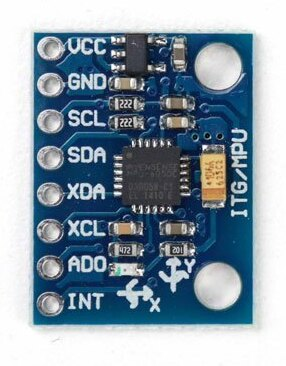
\includegraphics[width=0.3\textwidth]{images/modules/gy521img.jpg}
    \caption{Mòdul \est{GY521} \cite{gy521}.}
    \label{fig:gy521img}
\end{figure}

El circuit del mòdul \est{GY521} és lliure i es pot consultar a la figura
\ref{fig:gy521sch}. És prou senzill diferenciar la part utilitzada per a
convertir els 5V d'entrada en 3.3V per a alimentar a l'integrat de la resta
del circuit. Aquest mòdul també inclou un \acro{led} per a indicar que s'està
alimentant correctament.

Les connexions del lateral del mòdul fan molt còmode utilitzar-lo en entorns de
desenvolupament, on es connecten i desconnecten cables constantment. El fet
de disposar també d'un sistema funcional des d'un primer moment ajuda a
només centrar-se en la part de més alt nivell: l'aplicació del projecte.

\begin{figure}[ht]
    \centering
    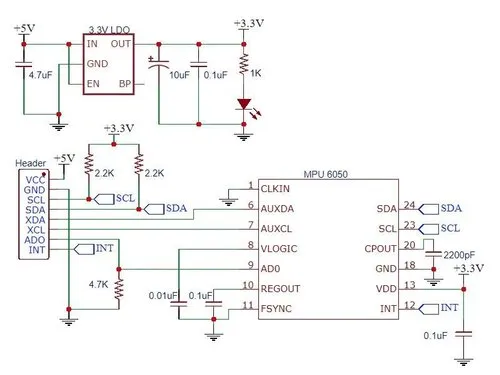
\includegraphics[width=0.6\textwidth]{images/modules/gy521sch.png}
    \caption{Esquema elèctric del mòdul \est{GY521} \cite{gy521}.}
    \label{fig:gy521sch}
\end{figure}

\section{Primer disseny}

En un primer moment es va decidir per utilitzar un microcontrolador que disposés
del perifèric \acro{usb} directament al maquinari, per a evitar programar-lo tot.
Tanmateix, es veurà que no s'acabarà utilitzant aquesta versió degut a motius
que s'explicaran més endavant. Dit això, s'ha decidit conservar aquest apartat
per a comprendre millor el procés de desenvolupament del projecte.

El microcontrolador que s'utilitzarà en aquesta versió és l'\acro{AtMega32u4}.
Aquest proporciona una interfície \acro{usb} integrada, i permet utilitzar la
interfície \acro{i2c} amb suficient facilitat. S'ha decidit utilitzar un
osci\l.lador extern per a generar un rellotge de freqüència
\SI[round-mode=places,round-precision=0]{16}{\mega\hertz}
al microcontrolador \cite{AtMega32u4}.

\subsection{Esquemàtic}

El disseny de l'esquemàtic es basa en el disseny del mòdul \est{GY521} i es pot
consultar a la figura \ref{fig:sch_v1}. Tret del que s'ha comentat en els paràgrafs
anteriors, la resta de components i connexions no deixen de ser les evidents per
a un circuit amb aquestes característiques. Tot i això, s'ha decidit posar
èmfasi en alguns detalls on s'hi ha parat més atenció:

\begin{figure}[ht]
    \centering
    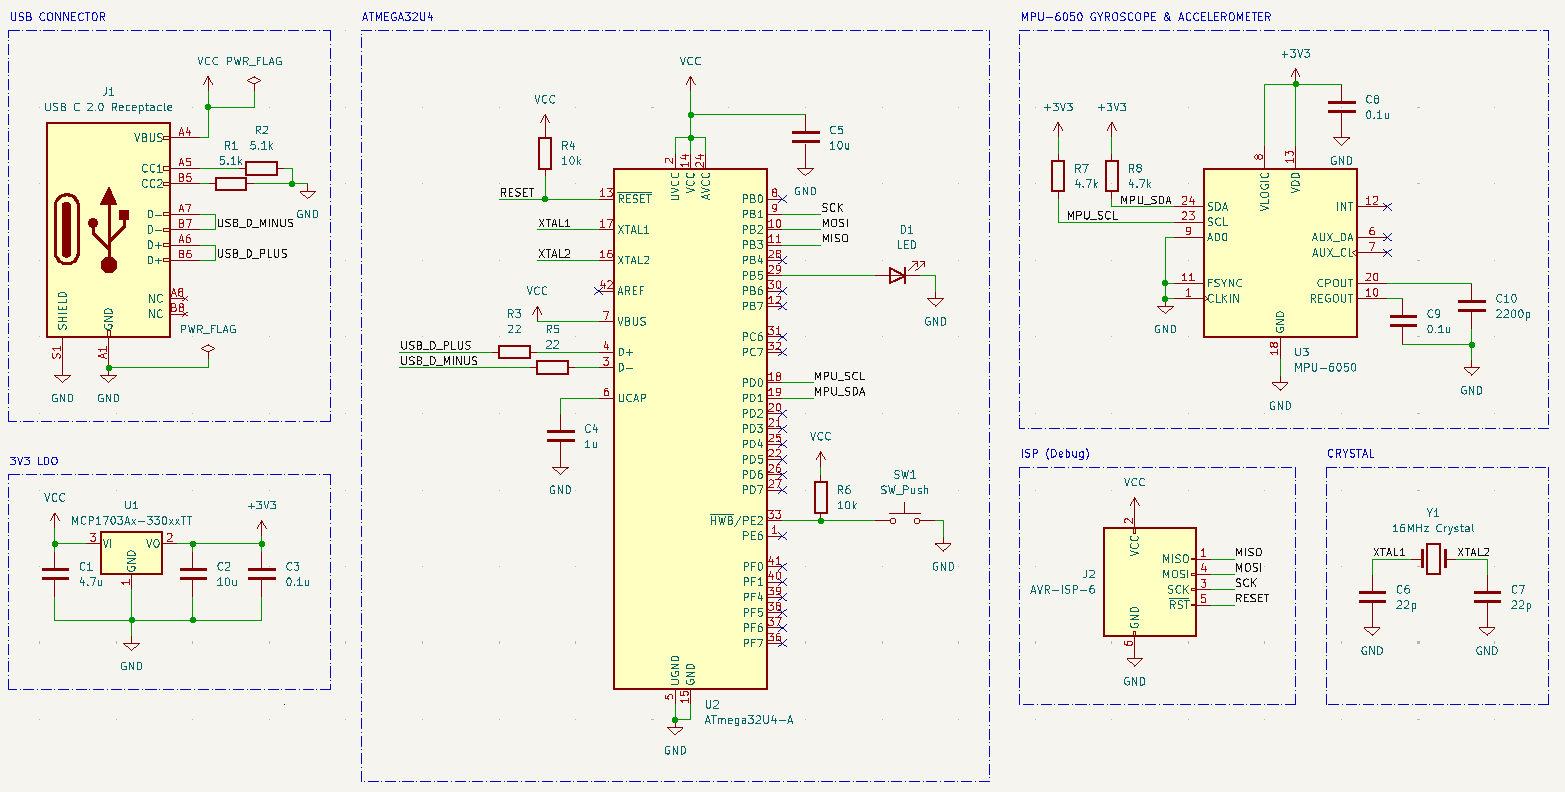
\includegraphics[width=0.9\textwidth]{images/kicad/gyro1_sch.png}
    \caption{Esquema elèctric de la primera versió.}
    \label{fig:sch_v1}
\end{figure}

\begin{itemize}
    \item Al costat de l'alimentació de cada integrat s'hi ha posat un
    condensador ceràmic de
    \SI[round-mode=places,round-precision=0]{10}{\micro\farad} o
    \SI[round-mode=places,round-precision=1]{0.1}{\micro\farad}
    (en funció del que recomanava
    cada fabricant al seu \est{datasheet}), per a assegurar-se que la tensió
    d'entrada és prou estable.
    \item S'ha hagut de posar un regulador lineal en el circuit, ja que el
    sensor necessita estar alimentat a
    \SI[round-mode=places,round-precision=1]{3.3}{\volt},
    però l'alimentació que proporciona
    el connector \acro{usb} és de \SI[round-mode=places,round-precision=0]{5}{\volt}.
    \item Al utilitzar un connector de tipus C, tot i comunicar-se amb
    \acro{usb2}, hi ha un parell de cables extres que determinen a quina tensió
    s'ha d'alimentar el dispositiu. Tal i com es comenta a \cite{Axelson2015USB}
    o a \cite{TypeCIntro}, si es desitja utilitzar una alimentació tradicional de 
    \SI[round-mode=places,round-precision=0]{5}{\volt} és suficient
    utilitzar dos \est{pull-downs} de
    \SI[round-mode=places,round-precision=1]{5.1}{\kilo\ohm}.
    \item El protocol \acro{i2c} necessita que les dues línies de comunicació
    estiguin amb \est{pull-ups}. Es veurà més endavant en el document el
    funcionament d'aquest protocol.
    \item L'esquema referent al cristall extern per al rellotge del microcontrolador
    és el recomanat pel fabricant en el mateix \est{datasheet} \cite{AtMega32u4}.
\end{itemize}

Cal destacar que, a diferència de la propera versió, aquest esquema sí que preveu
una connexió \acro{isp} per a programar la placa i un \acro{led} i polsador per
a interactuar d'una forma senzilla.

\subsection{Placa de circuit imprès}

Un cop acabat el disseny, utilitzant també el programa KiCad, es va començar a
crear la placa de circuit imprès. El procediment és prou senzill i es sol fer
de forma iterativa: crear un disseny molt dolent i anar-hi fent millores, fins
al punt on es considera que ja està prou bé (un disseny mai estarà perfecte).

A la figura \ref{fig:pcb_v1} es pot consultar la placa resultant. Com es pot veure,
no està del tot ben distribuida: això és perquè es va decidir canviar completament
de disseny abans d'haver-la acabat, i es va pensar que no valia la pena seguir
invertint temps amb un disseny que no veuria mai la llum.

\begin{figure}[ht]
    \centering
    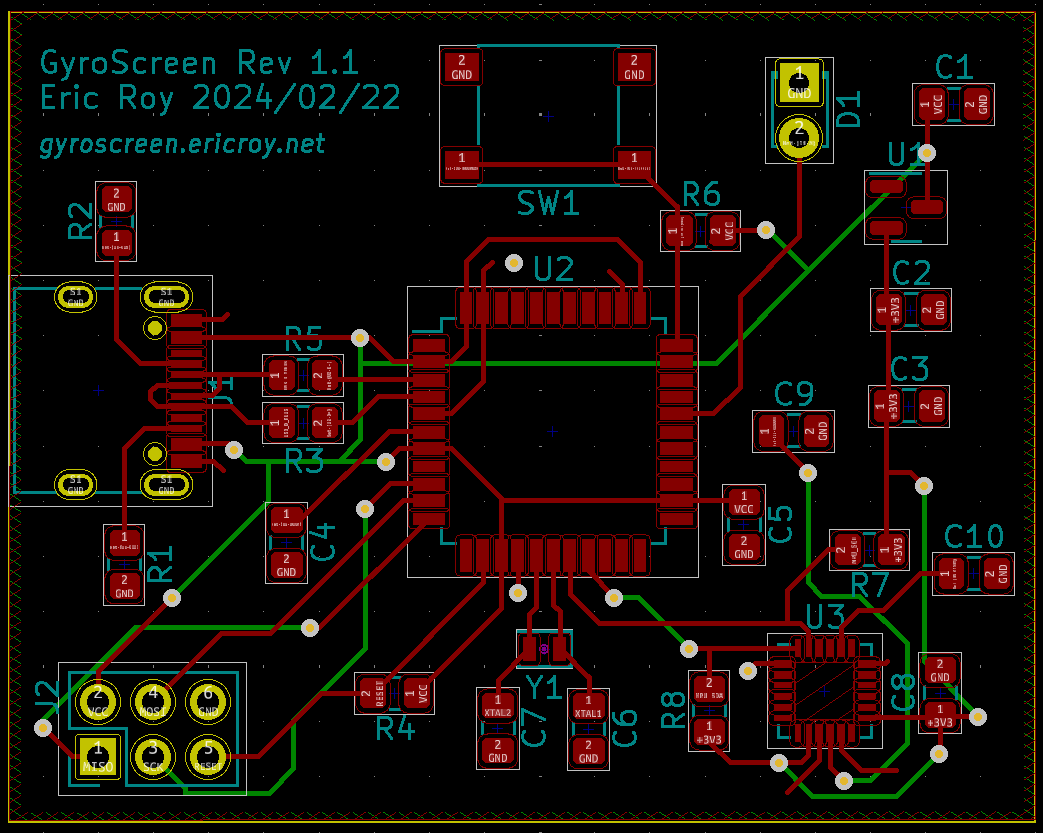
\includegraphics[width=0.8\textwidth]{images/kicad/gyro1_pcb.png}
    \caption{Placa de circuit imprès de la primera versió.}
    \label{fig:pcb_v1}
\end{figure}

\subsection{Problema del primer disseny}

Tal i com s'ha dit a l'apartat anterior, no es va acabar de dissenyar la placa
de circuit imprès degut al redisseny del \est{hardware}. El motiu es ben senzill,
no s'està utilitzant el microcontrolador adequat per al projecte.

Tal i com s'ha vist a l'esquemàtic, el microcontrolador només necessita 4 potes
per a informació (2 per \acro{usb} i 2 per \acro{i2c}). Això significa que es
deixaran al voltant de 20 entrades sense utilitzar. I no només això: aquest
microcontrolador disposa de molta més memòria de la que mai es necessitarà
\cite{AtMega32u4}.

El principal motiu per a fer el canvi és doncs el preu. Un \acro{AtMega32u4}
no és molt car \cite{AvrComparison}, però és més barat un dispositiu \acro{avr}
de la sèrie \acro{AtTinyXX}, com es veurà en el següent apartat.

\section{Segona versió de la placa}

Tal i com s'ha comentat al final de l'apartat anterior, s'ha decidit apostar
per un microcontrolador més econòmic i senzill degut als pocs requisits que
demana el sistema. Després de fer una mica de recerca s'ha descobert la
família de microcontroladors \acro{AtTinyX5}, on la X pot variar en funció de
la memòria \est{flash} disponible \cite{AtTiny85}.

Aquests microcontroladors disposen de 8 potes, de les quals 2 són per
l'alimentació. Així doncs, de les 6 potes disponibles encara en sobraran dues
per si es vol afegir algun perifèric extra. Per a aquesta versió del projecte,
però, s'ha decidit no donar-hi cap ús.

Tanmateix, abans de produir una placa de circuit imprès, hi havia interès en
poder provar el microcontrolador per a assegurar-se que seria possible
realitzar el sistema amb aquest darrer. A través de recerca i recomanacions del
personal del laboratori de l'escola es va prendre coneixement de l'existència de
la placa \est{Digispark}.

\subsection{Proves amb \est{Digispark}}
\label{subsec:hw_digispark}

La placa \est{Digispark} es pot comprar a preus molt reduïts i a molts llocs.
És una placa de circuit imprès equipada d'un \acro{AtTiny85}, un connector
\acro{usb}, algun component per a regular les tensions, i tot de pins per a
poder connectar fàcilment qualsevol cable i component al microcontrolador
\cite{Digispark}. A la figura \ref{fig:digispark} es pot veure l'aspecte físic
de la placa.

\begin{figure}[ht]
    \centering
    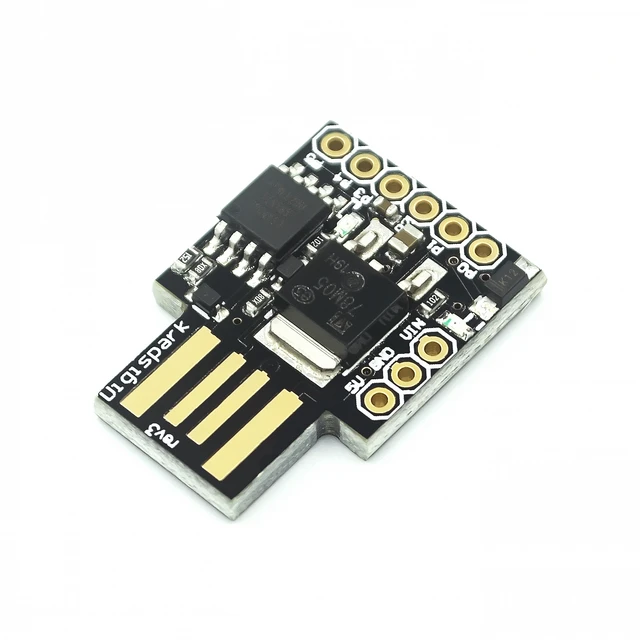
\includegraphics[width=0.3\textwidth]{images/modules/digisparkimg.png}
    \caption{Placa \est{Digispark} \cite{Digispark}.}
    \label{fig:digispark}
\end{figure}

Aquesta placa és de maquinari obert, i per tant, també es pot trobar fàcilment
el seu esquema elèctric. Es pot consultar a la Figura \ref{fig:digisparksch}
com el circuit és prou senzill, i només hi ha un parell de detalls que mereixen
la seva explicació, com podria ser l'ús de Díodes Zener. Es comentarà en el
moment del disseny del propi circuit.

\begin{figure}[ht]
    \centering
    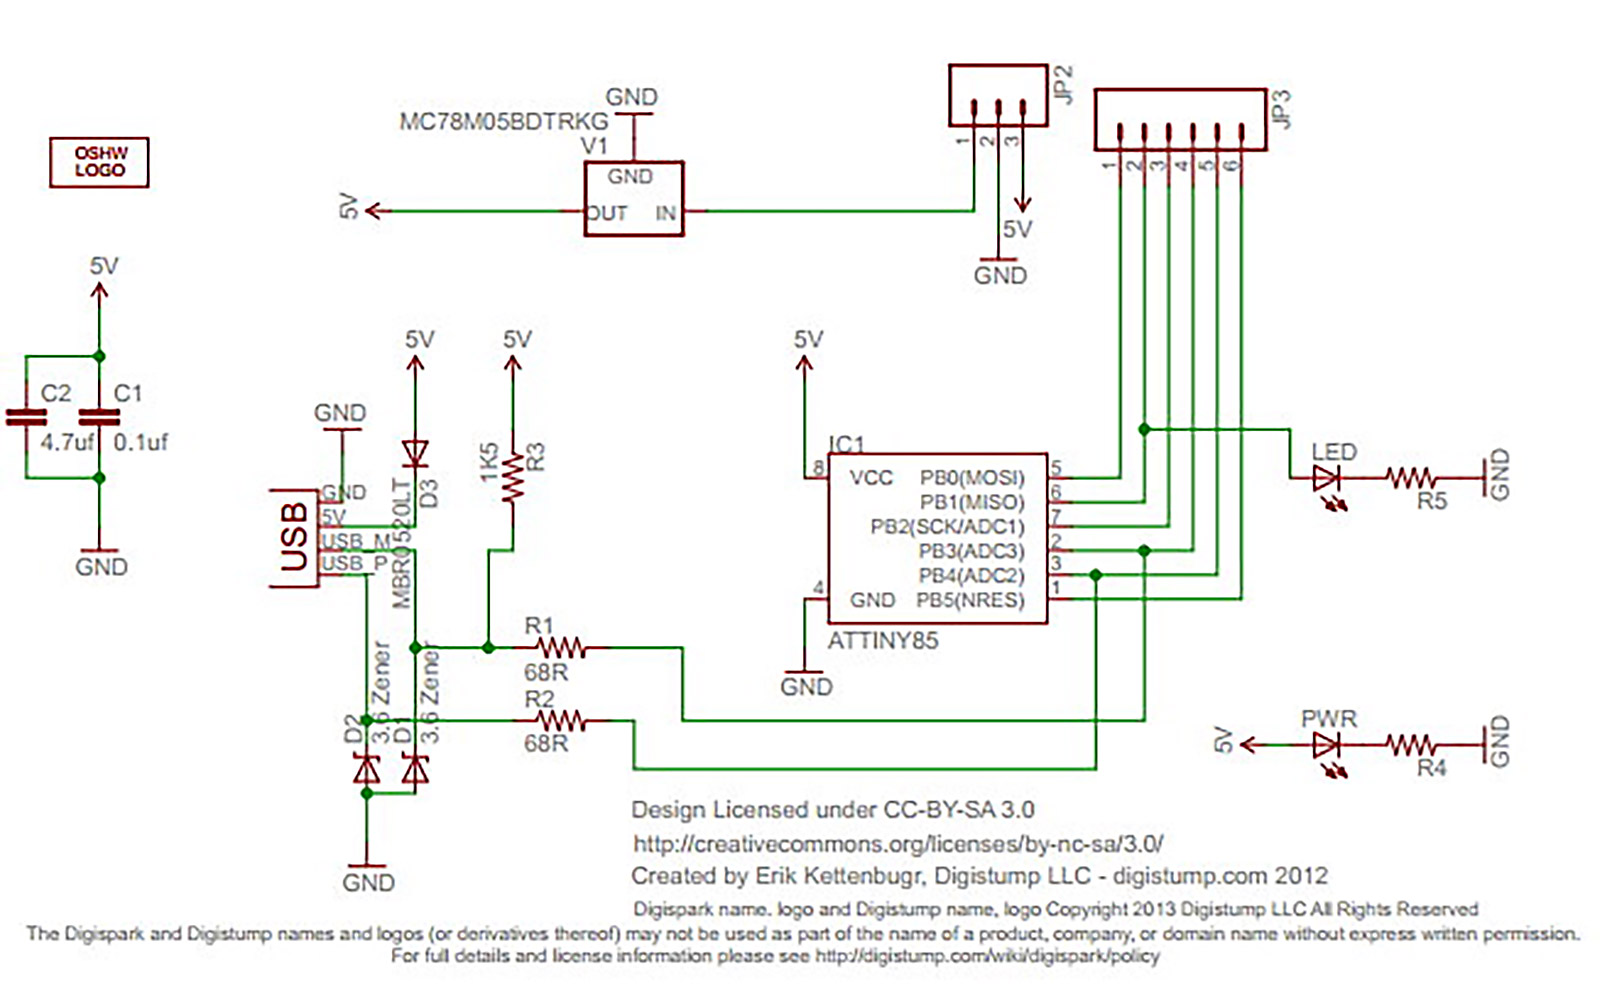
\includegraphics[width=0.8\textwidth]{images/modules/digisparksch.jpg}
    \caption{Diagrama de la placa \est{Digispark} \cite{Digispark}.}
    \label{fig:digisparksch}
\end{figure}

El microcontrolador ve programat amb un \est{bootloader} que utilitza la
llibreria \acro{v-usb} per a identificar-se com un port sèrie a l'ordinador
(és una de les sub-classes \est{hid}) i així poder programar-lo fàcilment.
És una placa bastant popular, de maquinari obert, i amb molta documentació i
tutorials disponibles per internet \cite{DigisparkBootloader}.

Es va adquirir un parell d'unitats d'aquesta placa, i es va connectar amb el
mòdul del sensor giroscopi. Mitjançant tutorials era senzill utilitzar la
placa \est{Digispark} com si d'un Arduino es tractés. Es podia, per exemple,
utilitzar la llibreria \est{LittleWire} per a comunicar-se amb el sensor amb el
protocol \acro{i2c} i llegir les dades necessaries.

Durant el transcurs d'aquestes proves també es va descobrir el projecte
\est{i2c\_tiny\_usb} \cite{I2cTinyUsb}. Aquest projecte ha aconseguit dissenyar una placa
molt semblant a la de \est{Digispark}, i mitjançant programari (tant del cantó
del microcontrolador com afegint contro\l.ladors al \est{kernel} de Linux),
el dispositiu s'identifica com un mestre \acro{i2c} de cara a l'ordinador, i
apareix a \fitx{/dev/i2c-X} on X és el nombre de dispositiu.

A \cite{i2cOnLittleWireBuilding} s'ha trobat una adaptació de
\est{i2c\_tiny\_usb} per a la placa \est{Digispark}, amb un tutorial molt
detallat sobre com programar la placa.
Aquest projecte ha anat molt bé per a fer proves de precisió del sensor a més
alt nivell (per exemple, utilitzant la llibreria \acro{i2c} de Python). Tanmateix,
es va descartar utilitzar-lo per a aquest treball per a dos motius:

\begin{itemize}
    \item Aquest projecte pretén ser el màxim de versàtil possible i utilitzar
    els estàndards de més alt nivell. En el capítol anterior s'ha comentat que
    es volia utilitzar les classes \acro{hid} i el mòdul \acro{iio}. El projecte
    \est{i2c\_tiny\_usb} utilitza programari propi, i tot i que estigui inclòs
    en el \est{kernel} de Linux \cite{I2cTinyKernel}, s'hauria de fer de zero per altres sistemes
    operatius.
    \item L'objectiu del projecte és aprendre durant el procés de desenvolupament.
    Si s'agafa un projecte que ja ho té tot fet no s'adquirirà experiència en
    aquests camps.
\end{itemize}

Així doncs, s'ha acabat utilitzant la placa \est{Digispark} per a validar
que el projecte es podria desenvolupar en aquest maquinari, i un cop es va
coneixer la bona notícia es va començar a desenvolupar la pròpia placa de circuit
imprès.

\subsection{Esquemàtic}

L'esquemàtic d'aquesta segona versió no té molts secrets. Consisteix en agafar
el circuit de la versió anterior i canviar tot el que té a veure amb l'antic
microcontrolador per al nou. S'ha utilitzat com a referència el circuit de la
placa \est{Digispark}, tenint en compte que algunes coses, com el regulador de
tensió extern, no son necessaries per a aquest projecte \cite{Digispark}.

En aquest nou circuit s'utilitza el rellotge intern del microcontrolador, que
ja s'ha vist que és suficient per a comunicar-se per \acro{usb}. Només hi ha
una novetat a comentar en aquesta segona versió, i és la presència de dos
díodes Zener en les línies d'\acro{usb}. El motiu rau en el protocol \acro{usb}:
tot i estar alimentat a \SI[round-mode=places,round-precision=0]{5}{\volt},
les línies de dades funcionen a
\SI[round-mode=places,round-precision=1]{3.3}{\volt}. Tal i com
s'ha comentat a l'apartat \ref{subsub:usb_physic}, els dos díodes asseguren
que la tensió mai supera aquest llindar.

\begin{figure}[ht]
    \centering
    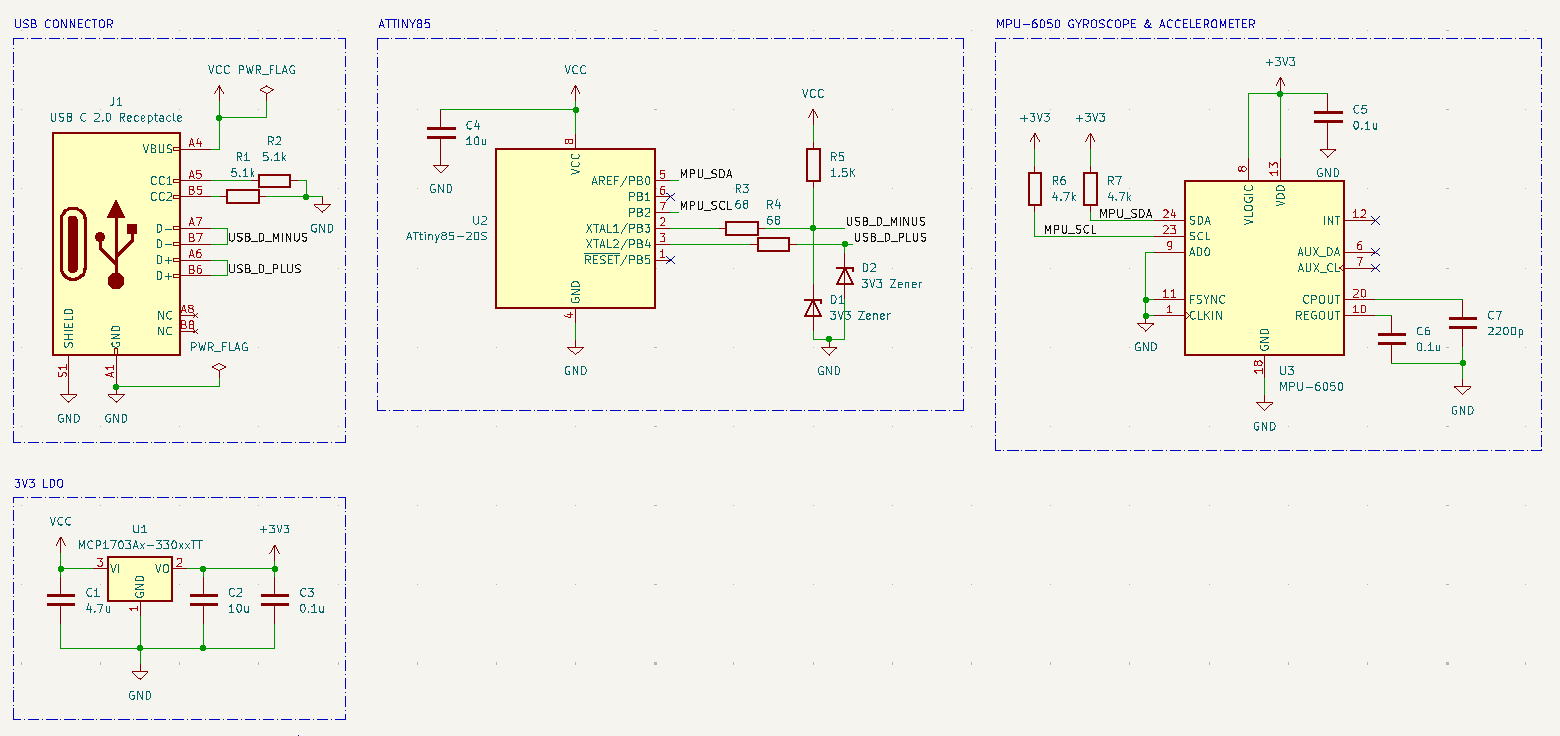
\includegraphics[width=1\textwidth]{images/kicad/gyro2_sch.png}
    \caption{Esquema elèctric de la segona versió.}
    \label{fig:sch_v2}
\end{figure}

Finalment, s'observa que en el diagrama de la figura \ref{fig:sch_v2}
no hi ha cap element amb el que una
persona pugui interactuar directament amb el dispositiu (polsador, llum, \dots).
Això és a propòsit, ja que es pretén que el dispositiu acabi tancat en una capsa
i que l'usuari no hagi de tocar-lo mai.

\subsection{Placa de circuit imprès}

Un cop creat l'esquema elèctric, s'ha pogut començar a dissenyar la placa de
circuit imprès, de la mateixa manera que amb la versió anterior. Una de les
tasques més difícils d'aquest procés és escollir \est{footprints} de components
que estiguin actualment en estoc, i assegurar-se que les línies de tensió
són una mica més gruixudes que la resta. A la figura \ref{fig:pcb_v2}
es pot veure el resultat
final d'aquest segon disseny.

\begin{figure}[ht]
    \centering
    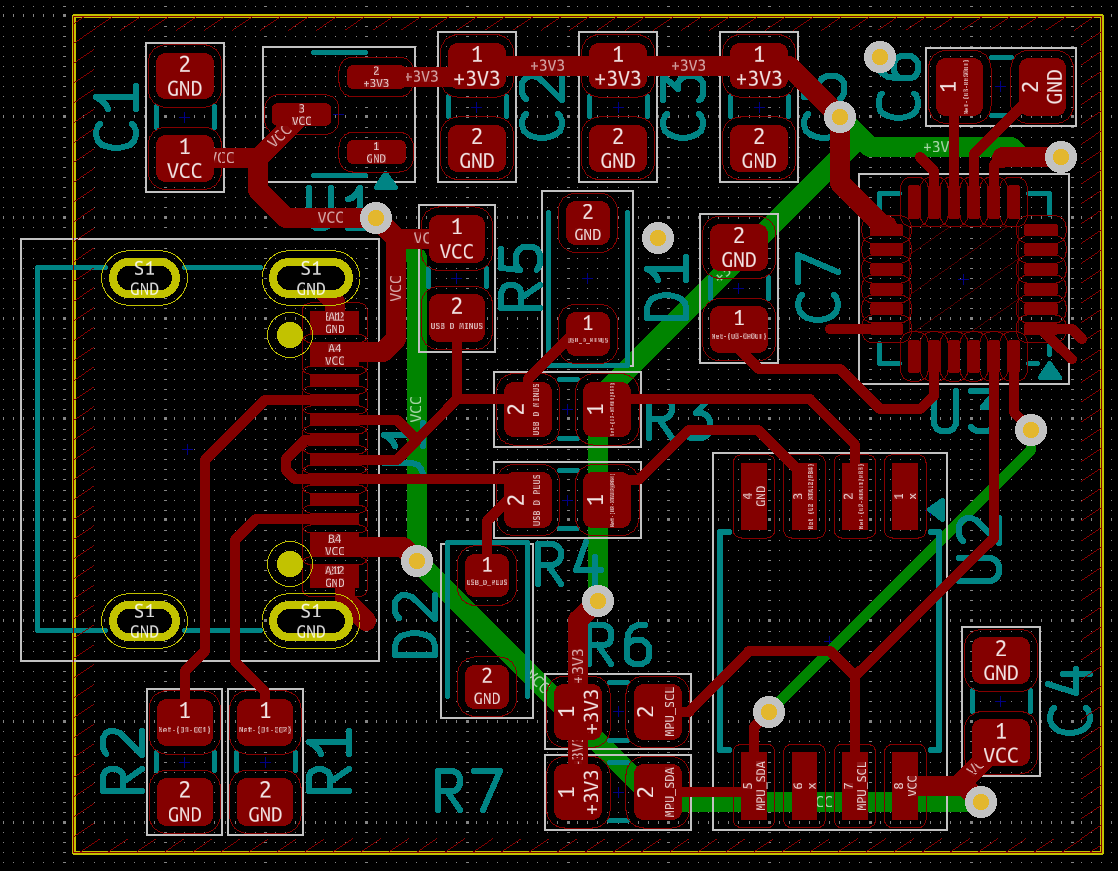
\includegraphics[width=0.75\textwidth]{images/kicad/gyro2_pcb.png}
    \caption{Placa de circuit imprès de la segona versió.}
    \label{fig:pcb_v2}
\end{figure}

S'ha utilitzat,
sempre que ha sigut possible, components amb \est{footprints} de dimensions 0805,
ja que amb aquesta mida es poden soldar a mà. Tot i que no s'ha previst afegir
manualment els components, el fet d'escollir aquestes mides és una assegurança
que si s'espatlla o es crema algun component, aquest es podrà canviar.
Evidentment, en un disseny per a produir-se en massa es pot reduir la mida dels
components.

Com que a la part de darrere de la placa només hi ha d'anar un parell de vies,
però cap component, s'ha decidit afegir-hi els crèdits del projecte: autor,
titulació, logos de l'escola i de maquinari lliure, i enllaç a una possible
pàgina web.

Tot i haver parat atenció amb els components, es veurà en el següent apartat que
l'empresa amb qui s'ha encarregat la producció de la placa no tenia disponibles
alguns d'aquests. Així doncs, s'ha hagut de fer una nova revisió amb petites
modificacions d'alguns components.

\subsection{Producció de la pcb}

Amb la placa de circuit imprès ja preparada, només faltava produir-ne algunes
unitats. Per recomanacions de la universitat s'ha optat per utilitzar el
proveïdor \acro{jlcpcb}. Aquest ofereix bons preus, entrega del producte en pocs
dies i també té el servei de muntatge de la placa (és a dir, soldar-hi tots els
components) \cite{JlcPcb}.

Degut al poc talent i ganes que hi havia en soldar un per un els components, i
sabent que alguns són molt petits i seria senzill cometre errors, s'ha optat
per delegar aquesta tasca al proveïdor. Evidentment, el cost de muntatge ha
sigut el més elevat de tota la comanda, però imprimir i muntar 5 plaques
ha sortit per menys de \SI[round-mode=places,round-precision=0]{100}{\EUR},
enviament i \acro{iva} inclosos.

\begin{figure}[ht]
    \centering
    \begin{subfigure}{0.45\textwidth}
        \centering
        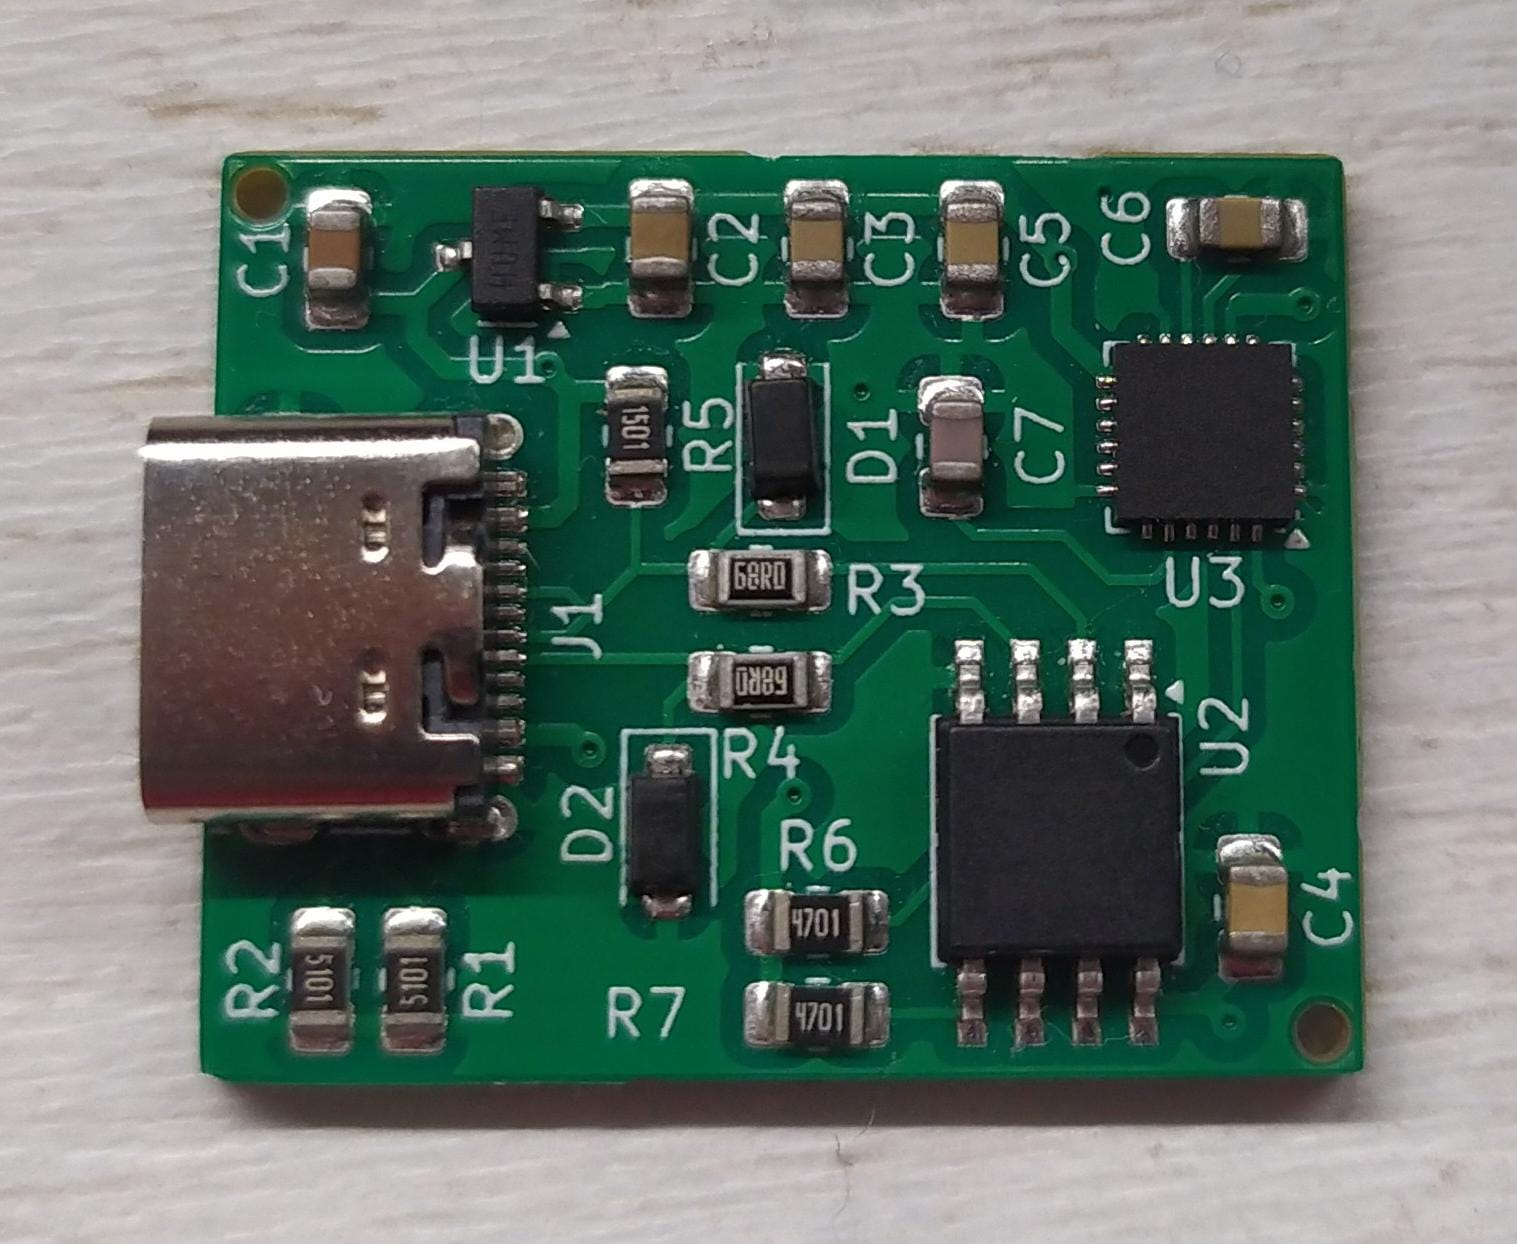
\includegraphics[width=0.9\textwidth]{images/device/top.jpeg}
        \caption{Cara superior.}
        \label{fig:printedpcb_top}
    \end{subfigure}
    \begin{subfigure}{0.45\textwidth}
        \centering
        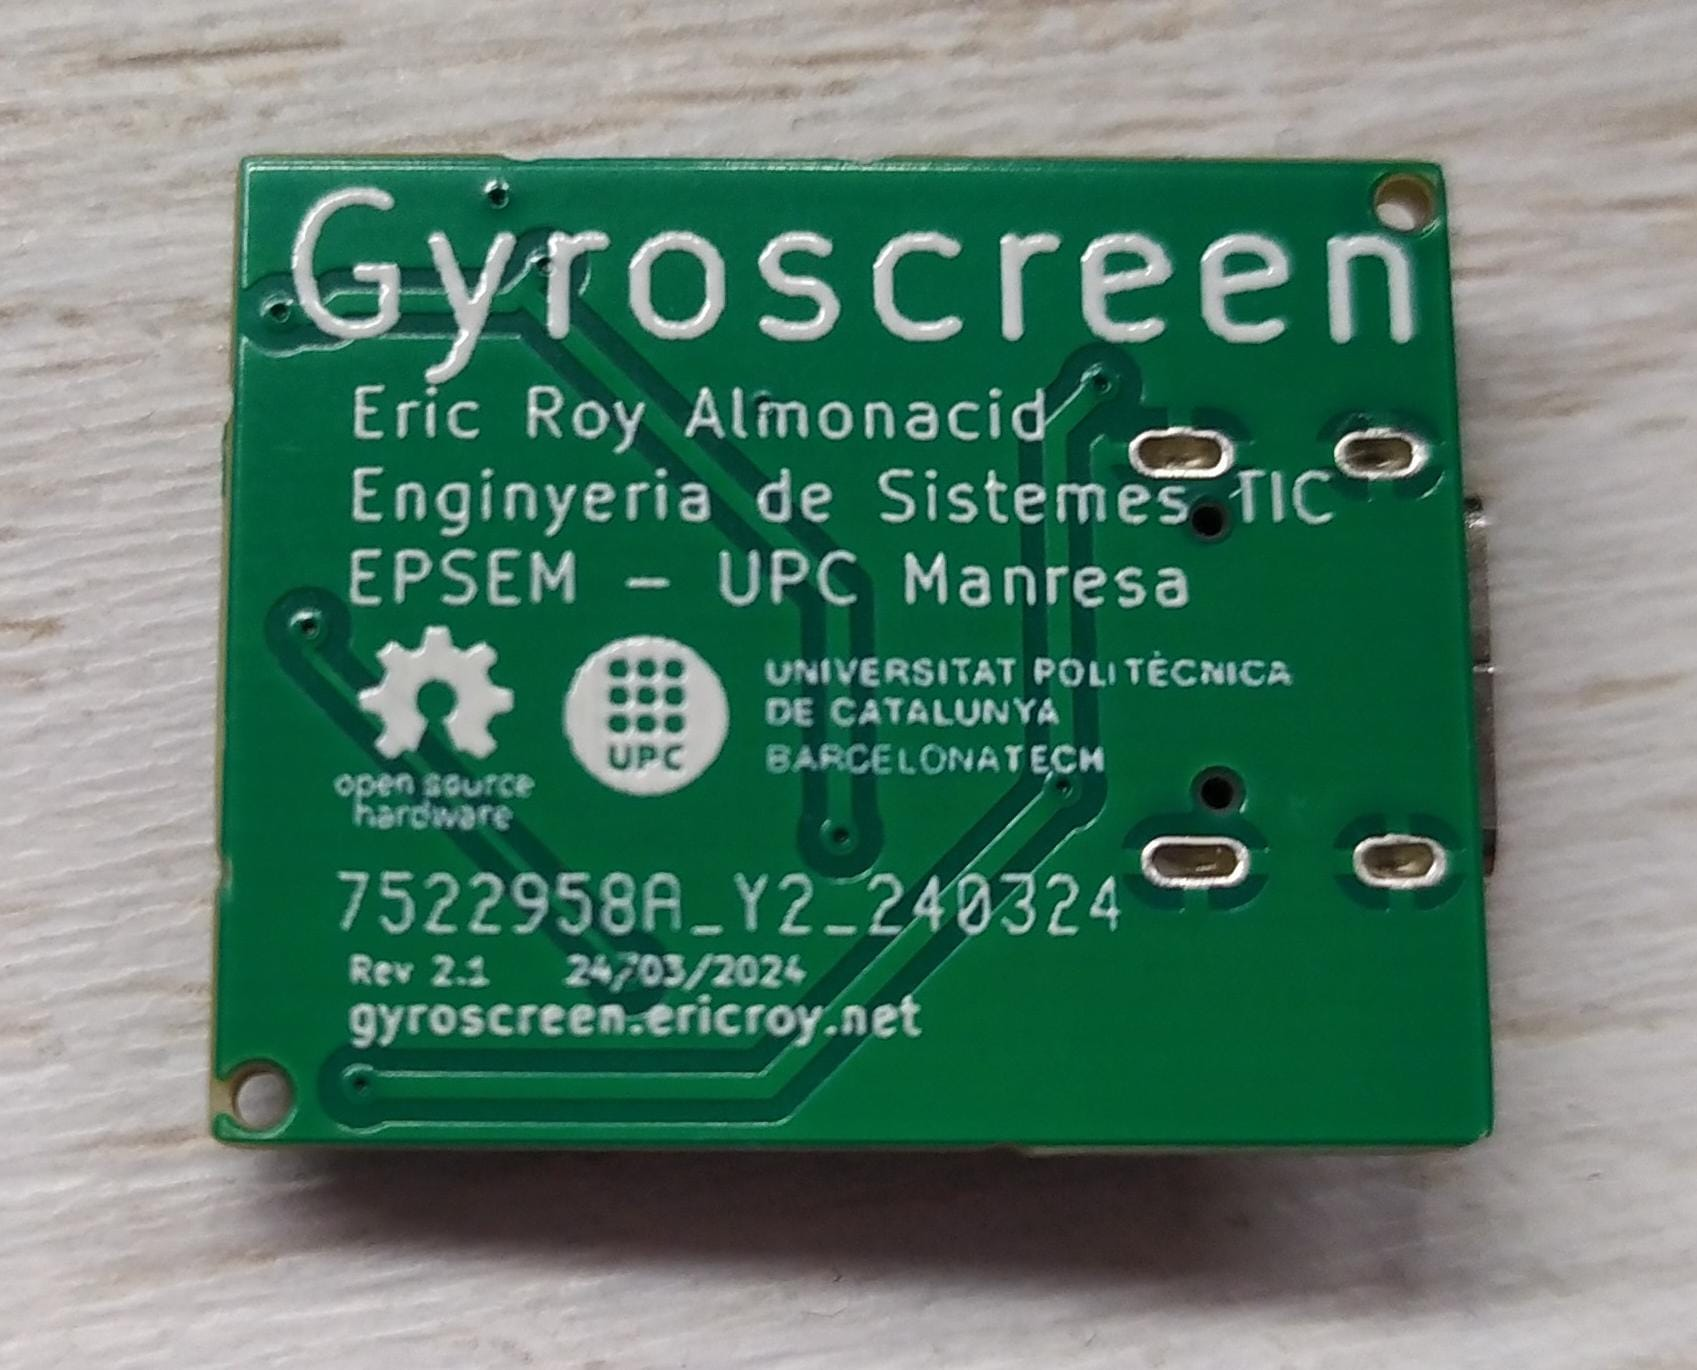
\includegraphics[width=0.9\textwidth]{images/device/bottom.jpeg}
        \caption{Cara inferior.}
        \label{fig:printedpcb_bottom}
    \end{subfigure}
    \caption{Placa de circuit imprès del projecte.}
    \label{fig:printedpcb}
\end{figure}

El resultat final ha quedat molt professional i es pot veure a la figura
\ref{fig:printedpcb}. Es pot veure també com s'ha aprofitat la cara inferior
per a afegir els crèdits del projecte. Tanmateix, el camí per a arribar fins
a aquests resultats no ha sigut senzill.

En primer lloc, \acro{jlcpcb} demana la \acro{bom} (\est{Bill Of Materials})
del circuit, i les posicions i orientacions de cada component. Resulta que el
seu sistema no és completament compatible amb els fitxers que exporta
KiCad. Ha sigut gràcies a un tutorial de la seva pròpia pàgina web que s'ha
acabat aconseguint el format demanat dels fitxers \cite{KiCADJLC}.

\section{Encapsulat}

Quan es va saber que la placa impresa ja no rebria més modificacions físiques,
es va decidir crear una petita carcassa per a evitar que hi entri pols o les
ditades el puguin fer malbé. En un futur, aquesta carcassa també podrà protegir
al dispositiu d'altres agents externs, però en el moment del disseny l'objectiu
era tenir cura del dispositiu durant la fase de desenvolupament.

Així doncs, es va utilitzar el programa \est{FreeCAD} per a dissenyar una
carcassa amb dues peces: una superior i una inferior. Aquestes encaixarien entre
sí i, amb l'ajuda de cola quedarien subjectes. Les mesures s'han pres a partir
del model de \est{KiCad}, però també s'han corroborat amb la placa física i un
peu de rei.

A la figura \ref{fig:3d_freecad} es poden veure les dues parts dissenyades. Com es pot
apreciar, només s'hi ha deixat un forat per a permetre el pas del connector
\acro{usb}. S'ha utilitzat parets de \SI{1.5}{\milli\meter}, i un marge entre
les dues peces de \SI{0.25}{\milli\meter}.

\begin{figure}[ht]
    \centering
    \begin{subfigure}{0.40\textwidth}
        \centering
        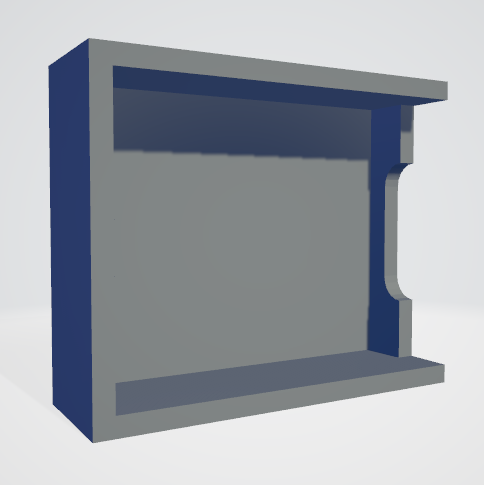
\includegraphics[width=0.9\textwidth]{images/freecad/3d_bottom.png}
        \caption{Part inferior.}
        \label{fig:3d_freecad_bottom}
    \end{subfigure}
    \begin{subfigure}{0.4\textwidth}
        \centering
        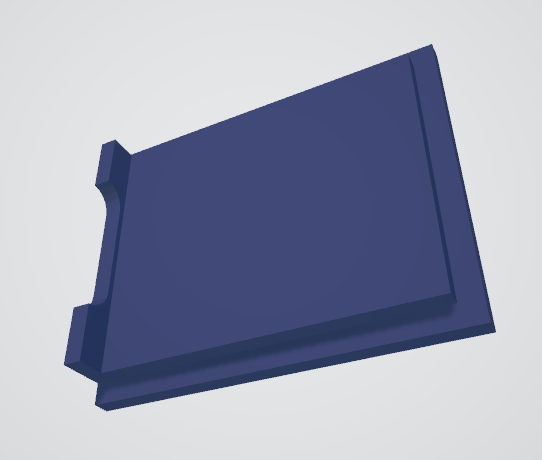
\includegraphics[width=0.9\textwidth]{images/freecad/3d_top.png}
        \caption{Part superior.}
        \label{fig:3d_freecad_top}
    \end{subfigure}
    \caption{Disseny 3D de l'encapsulat.}
    \label{fig:3d_freecad}
\end{figure}

Es va aconseguir imprimir les dues peces amb una de les impressores de
l'escola, i es va aconseguir el resultat que es pot apreciar a la figura
\ref{fig:3d_real}. Finalment, es va comprovar que totes les peces encaixaven a la
perfecció i la placa cabia a dintre de la carcassa.

\begin{figure}[ht]
    \centering
    \begin{subfigure}{0.50\textwidth}
        \centering
        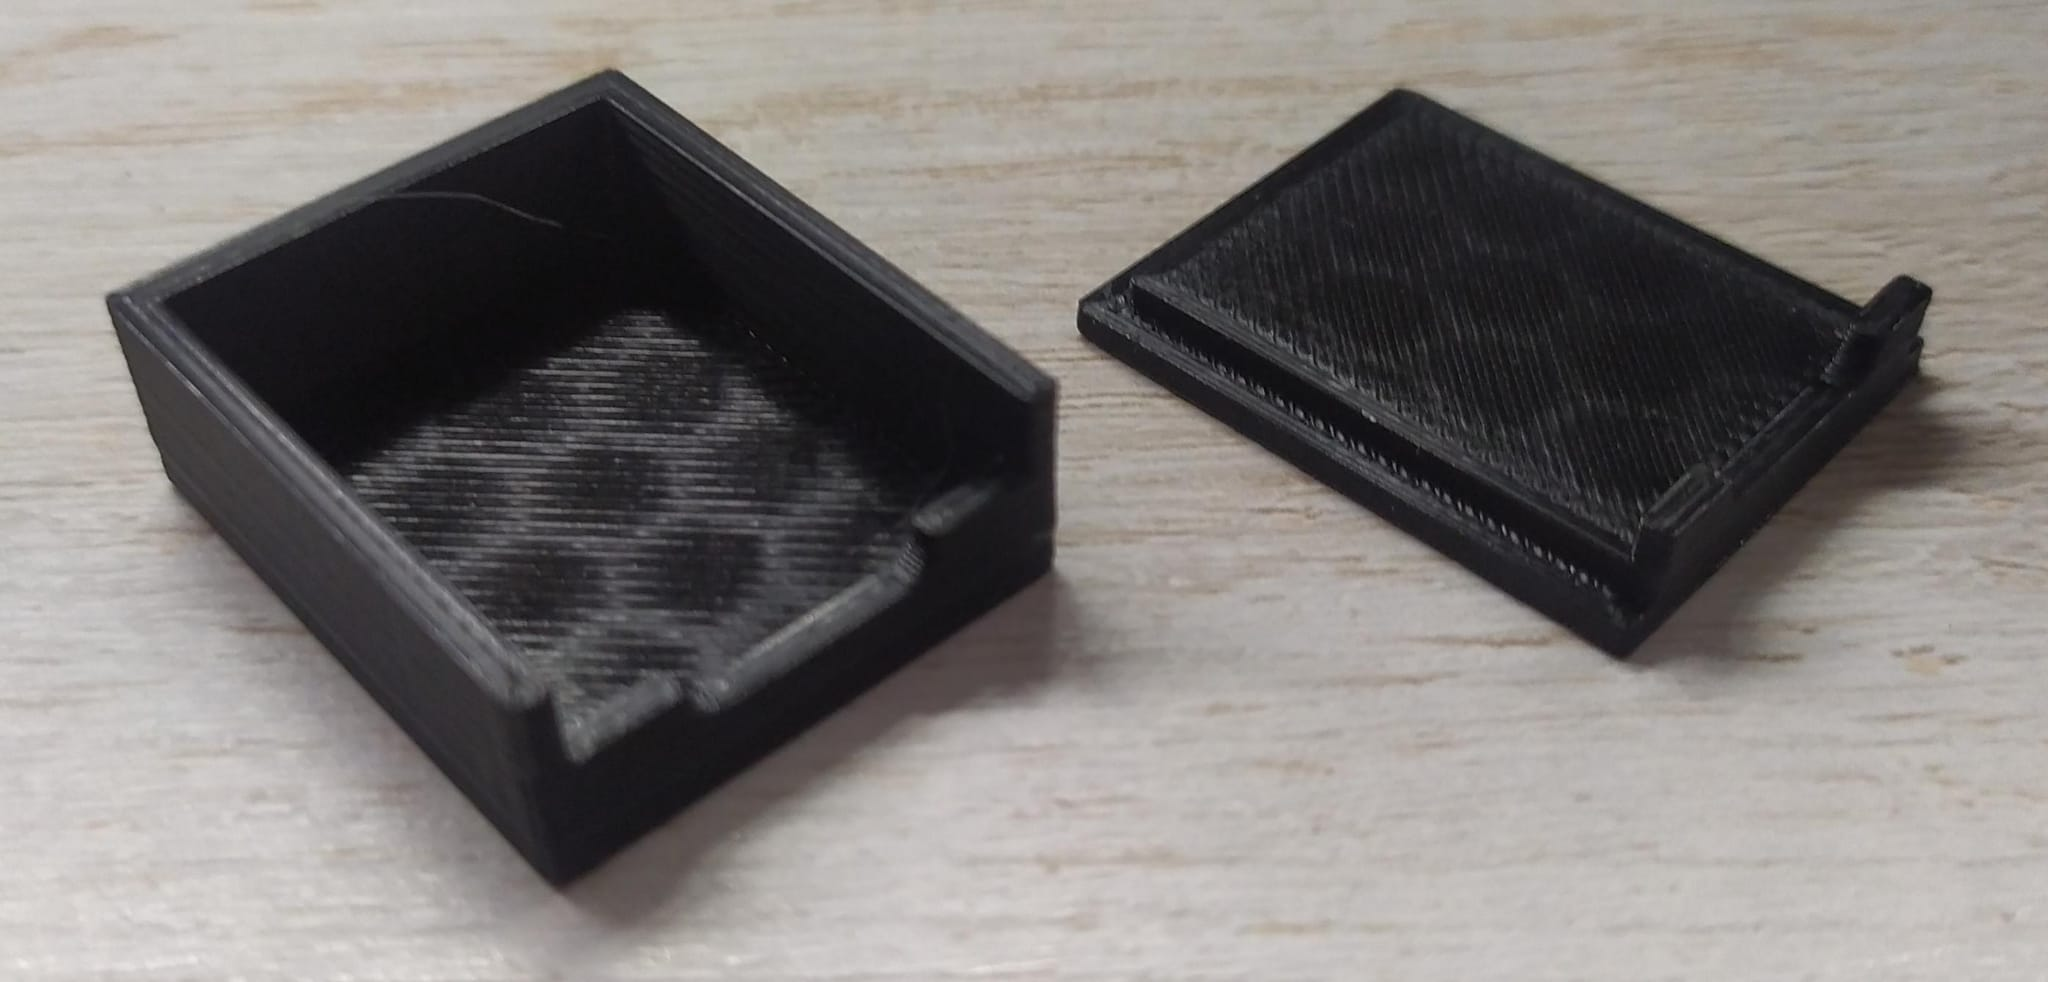
\includegraphics[width=0.9\textwidth]{images/device/3d_unmounted.jpeg}
        \caption{Sense muntar.}
        \label{fig:3d_real_unmounted}
    \end{subfigure}
    \begin{subfigure}{0.4\textwidth}
        \centering
        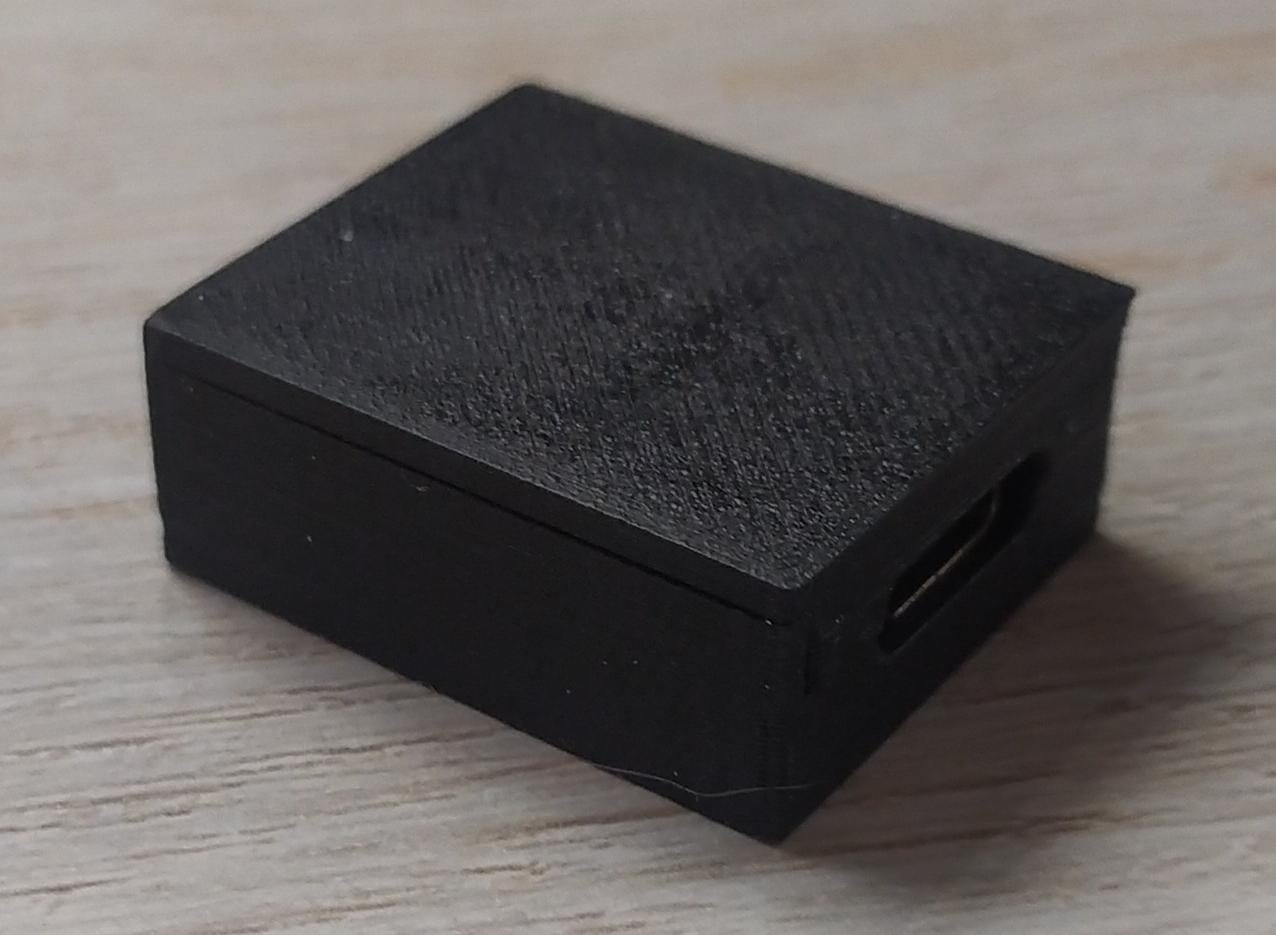
\includegraphics[width=0.9\textwidth]{images/device/3d_mounted.jpeg}
        \caption{Muntat.}
        \label{fig:3d_real_mounted}
    \end{subfigure}
    \caption{Disseny 3D de l'encapsulat.}
    \label{fig:3d_real}
\end{figure}

\section{OSHWA}

Un cop es va saber que el disseny físic del projecte era definitiu, es va decidir
publicar-lo a \acro{oshwa}. L'\est{Open-Source HardWare Association} és, com el
nom indica, una associació que vetlla pel maquinari de codi obert. Una de les
diverses tasques que fa és mantenir un registre de dissenys de maquinari obert,
sempre que els autors ho autoritzin \cite{Oshwa}.

Un dels beneficis de registrar el disseny en el seu sistema és que queda una
evidència (més) que el projecte s'ha fet, té la llicència que té, i protegeix
a l'autor contra possibles plagis. El més interessant de tot això és que aquest
servei s'ofereix gratuïtament: l'associació accepta donacions, però no son
necessàries per a poder registrar un disseny.

Així doncs, es va registrar el dispositiu a la seva base de dades i, després
de omplir el formulari i aquest ser revisat per l'associació, el dispositiu
va ser acceptat i es troba actualment sota la llicència \verb|ES000045|.
A la figura \ref{fig:oshwa} es troba el logo que es pot incloure al projecte,
com a resultat d'aquesta certificació.

\begin{figure}[ht]
    \centering
    
\includegraphics[width=0.5\textwidth]{images/oshwa.png}
    \caption{Certificació \acro{oshwa} obtinguda per al projecte.}
    \label{fig:oshwa}
\end{figure}

